\section{An efficiency metric}

\begin{frame}{A new metric (1)}

    \begin{mdframed}[style=box]
        $$Eff(m,t,p) = \exp^{-\log \left( \dfrac{m}{p+t}\right)}, \;\text{where}$$
    \end{mdframed}

    \vspace{0.5cm}
    
    $p \rightarrow \text{number of parameters in the model},$
    $t \rightarrow \text{time for running the algorithm/model}$
    $m \rightarrow \text{any known metric like F-1, mse etc.}$
    
    \vspace{0.5cm}
    
    \textbf{Note: }The metric should be adapted in function of the known original metric
    
\end{frame}

%%%%%%%%%%%%%%%%%%%%%%%%%%%%%%%%%%%%%%%%%%%%%%%%%%%%%%%%

\begin{frame}{A new metric (2)}
    
    \vspace{0.2cm}

    \begin{mdframed}[style=box]
        $$Eff(m,t,p) = \exp^{-\log \left( \dfrac{m}{p+t}\right)}, \;\text{where}$$
    \end{mdframed}
    
    \vspace{0.2cm}

    \begin{columns} % Another exemple of presentation in two columns
        \begin{column}{0.5\textwidth}
            \center
            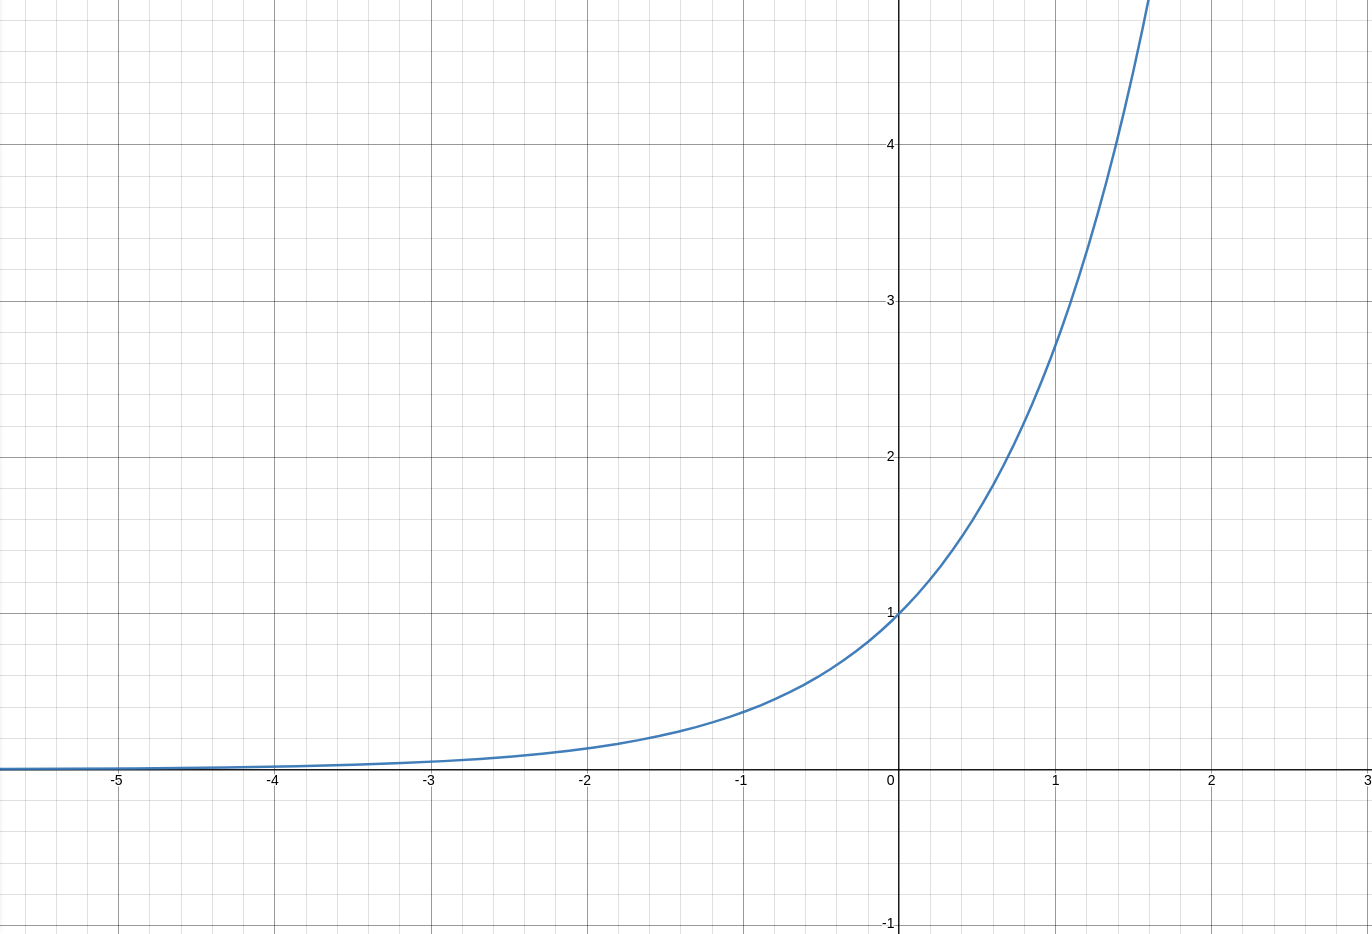
\includegraphics[scale=0.075]{img/exp.png}

            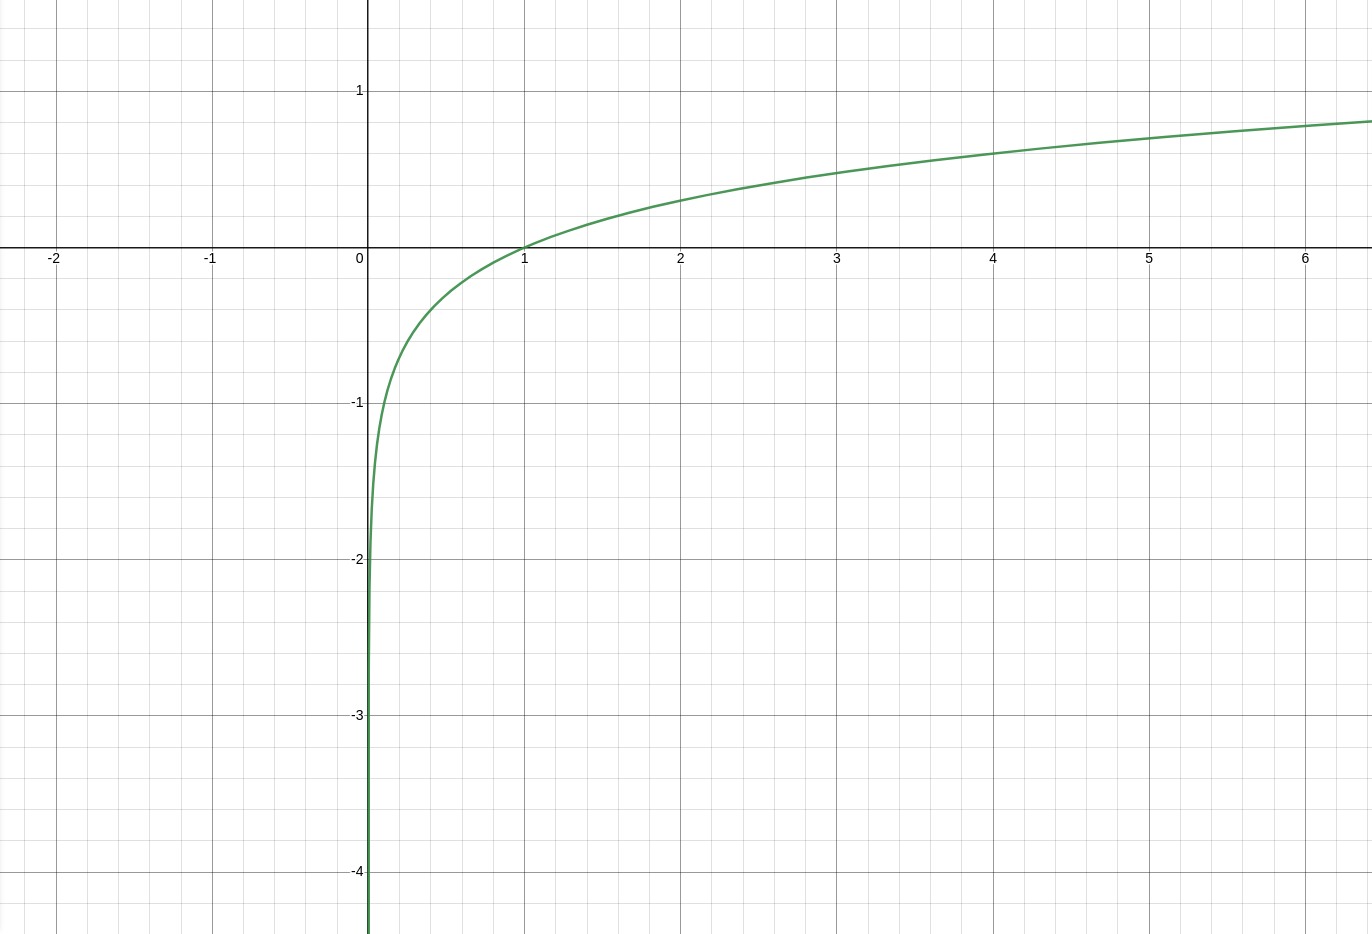
\includegraphics[scale = 0.075]{img/log.png}
        \end{column}
        \begin{column}{0.5\textwidth}
            \vspace{-1cm}
            \center
            $$p \to \infty \Rightarrow \text{metric}_{\text{new}} \to \infty$$
            $$t \to \infty \Rightarrow \text{metric}_{\text{new}} \to \infty$$
            $$m \to \infty \Rightarrow \text{metric}_{\text{new}} \to 0$$
        \end{column}
    \end{columns}
    
\end{frame}